\documentclass[12pt]{article}
\usepackage{listings}
\usepackage{color}
\usepackage{xcolor}

\usepackage{xparse}

\usepackage{graphicx}
\graphicspath{ {.} }

\NewDocumentCommand{\codeword}{v}{%
	\texttt{\textcolor{blue}{#1}}%
}

\definecolor{dkgreen}{rgb}{0,0.6,0}
\definecolor{gray}{rgb}{0.5,0.5,0.5}
\definecolor{mauve}{rgb}{0.58,0,0.82}

\lstset{frame=tb,
	language=Java,
	aboveskip=3mm,
	belowskip=3mm,
	showstringspaces=false,
	columns=flexible,
	basicstyle={\small\ttfamily},
	numbers=none,
	numberstyle=\tiny\color{gray},
	keywordstyle=\color{blue},
	commentstyle=\color{dkgreen},
	stringstyle=\color{mauve},
	breaklines=true,
	breakatwhitespace=true,
	tabsize=3
}

\newenvironment{solution}[1][]{
	\vspace{10px}\noindent\emph{Solution #1}
}{
	\vspace{10px}
}

\begin{document}

	\section*{Part I}
	
	\subsection*{Problem 1} Create a variable \codeword{phrase} containing a list of words. Review the operations described in the previous chapter, including addition, multiplication, indexing, slicing, and sorting.  
	
	Addition:
		\begin{lstlisting}
	phrase = ['sandwiches', 'are', 'very', 'tasty']
	>>> phrase = phrase + ['!']
	>>> phrase
	['sandwiches', 'are', 'very', 'tasty', '!']
	\end{lstlisting}
	Indexing
	\begin{lstlisting}
	>>> phrase[0]
	'sandwiches'
	\end{lstlisting}
	Slicing
	\begin{lstlisting}
	>>> phrase[2:4]
	['very', 'tasty']
	\end{lstlisting}
	Sorting:
	\begin{lstlisting}
	>>> words = sorted(phrase)
	>>> words
	['!', 'are', 'sandwiches', 'tasty', 'veryvery']
	\end{lstlisting}
	Multiplication:
		\begin{lstlisting}
>>> phrase[2] = phrase[2] * 2
>>> phrase
['sandwiches', 'are', 'veryvery', 'tasty', '!']
	\end{lstlisting}
	
	\subsection*{Problem 2}  Use the corpus module to explore austen-persuasion.txt. How many word tokens does this book have? How many word types?
	\begin{lstlisting}
	>>> persuasion = nltk.corpus.gutenberg.words('austen-persuasion.txt')
	>>> persuasion
	['[', 'Persuasion', 'by', 'Jane', 'Austen', '1818', ...]
	>>> len(persuasion)
	98171
	>>> len(set(persuasion))
	6132
	\end{lstlisting}
	
	\subsection*{Problem 3} Use the Brown corpus reader nltk.corpus.brown.words() or the Web text corpus reader nltk.corpus.webtext.words() to access some sample text in two different genres.
	\begin{lstlisting}
	>>> nltk.corpus.brown.words()
	['The', 'Fulton', 'County', 'Grand', 'Jury', 'said', ...]
	>>> nltk.corpus.webtext.words()
	['Cookie', 'Manager', ':', '"', 'Don', "'", 't', ...]
	\end{lstlisting}
	
	\subsection*{Problem 4} Read in the texts of the State of the Union addresses, using the \codeword{state_union} corpus reader. Count occurrences of men, women, and people in each document. What has happened to the usage of these words over time?
	
	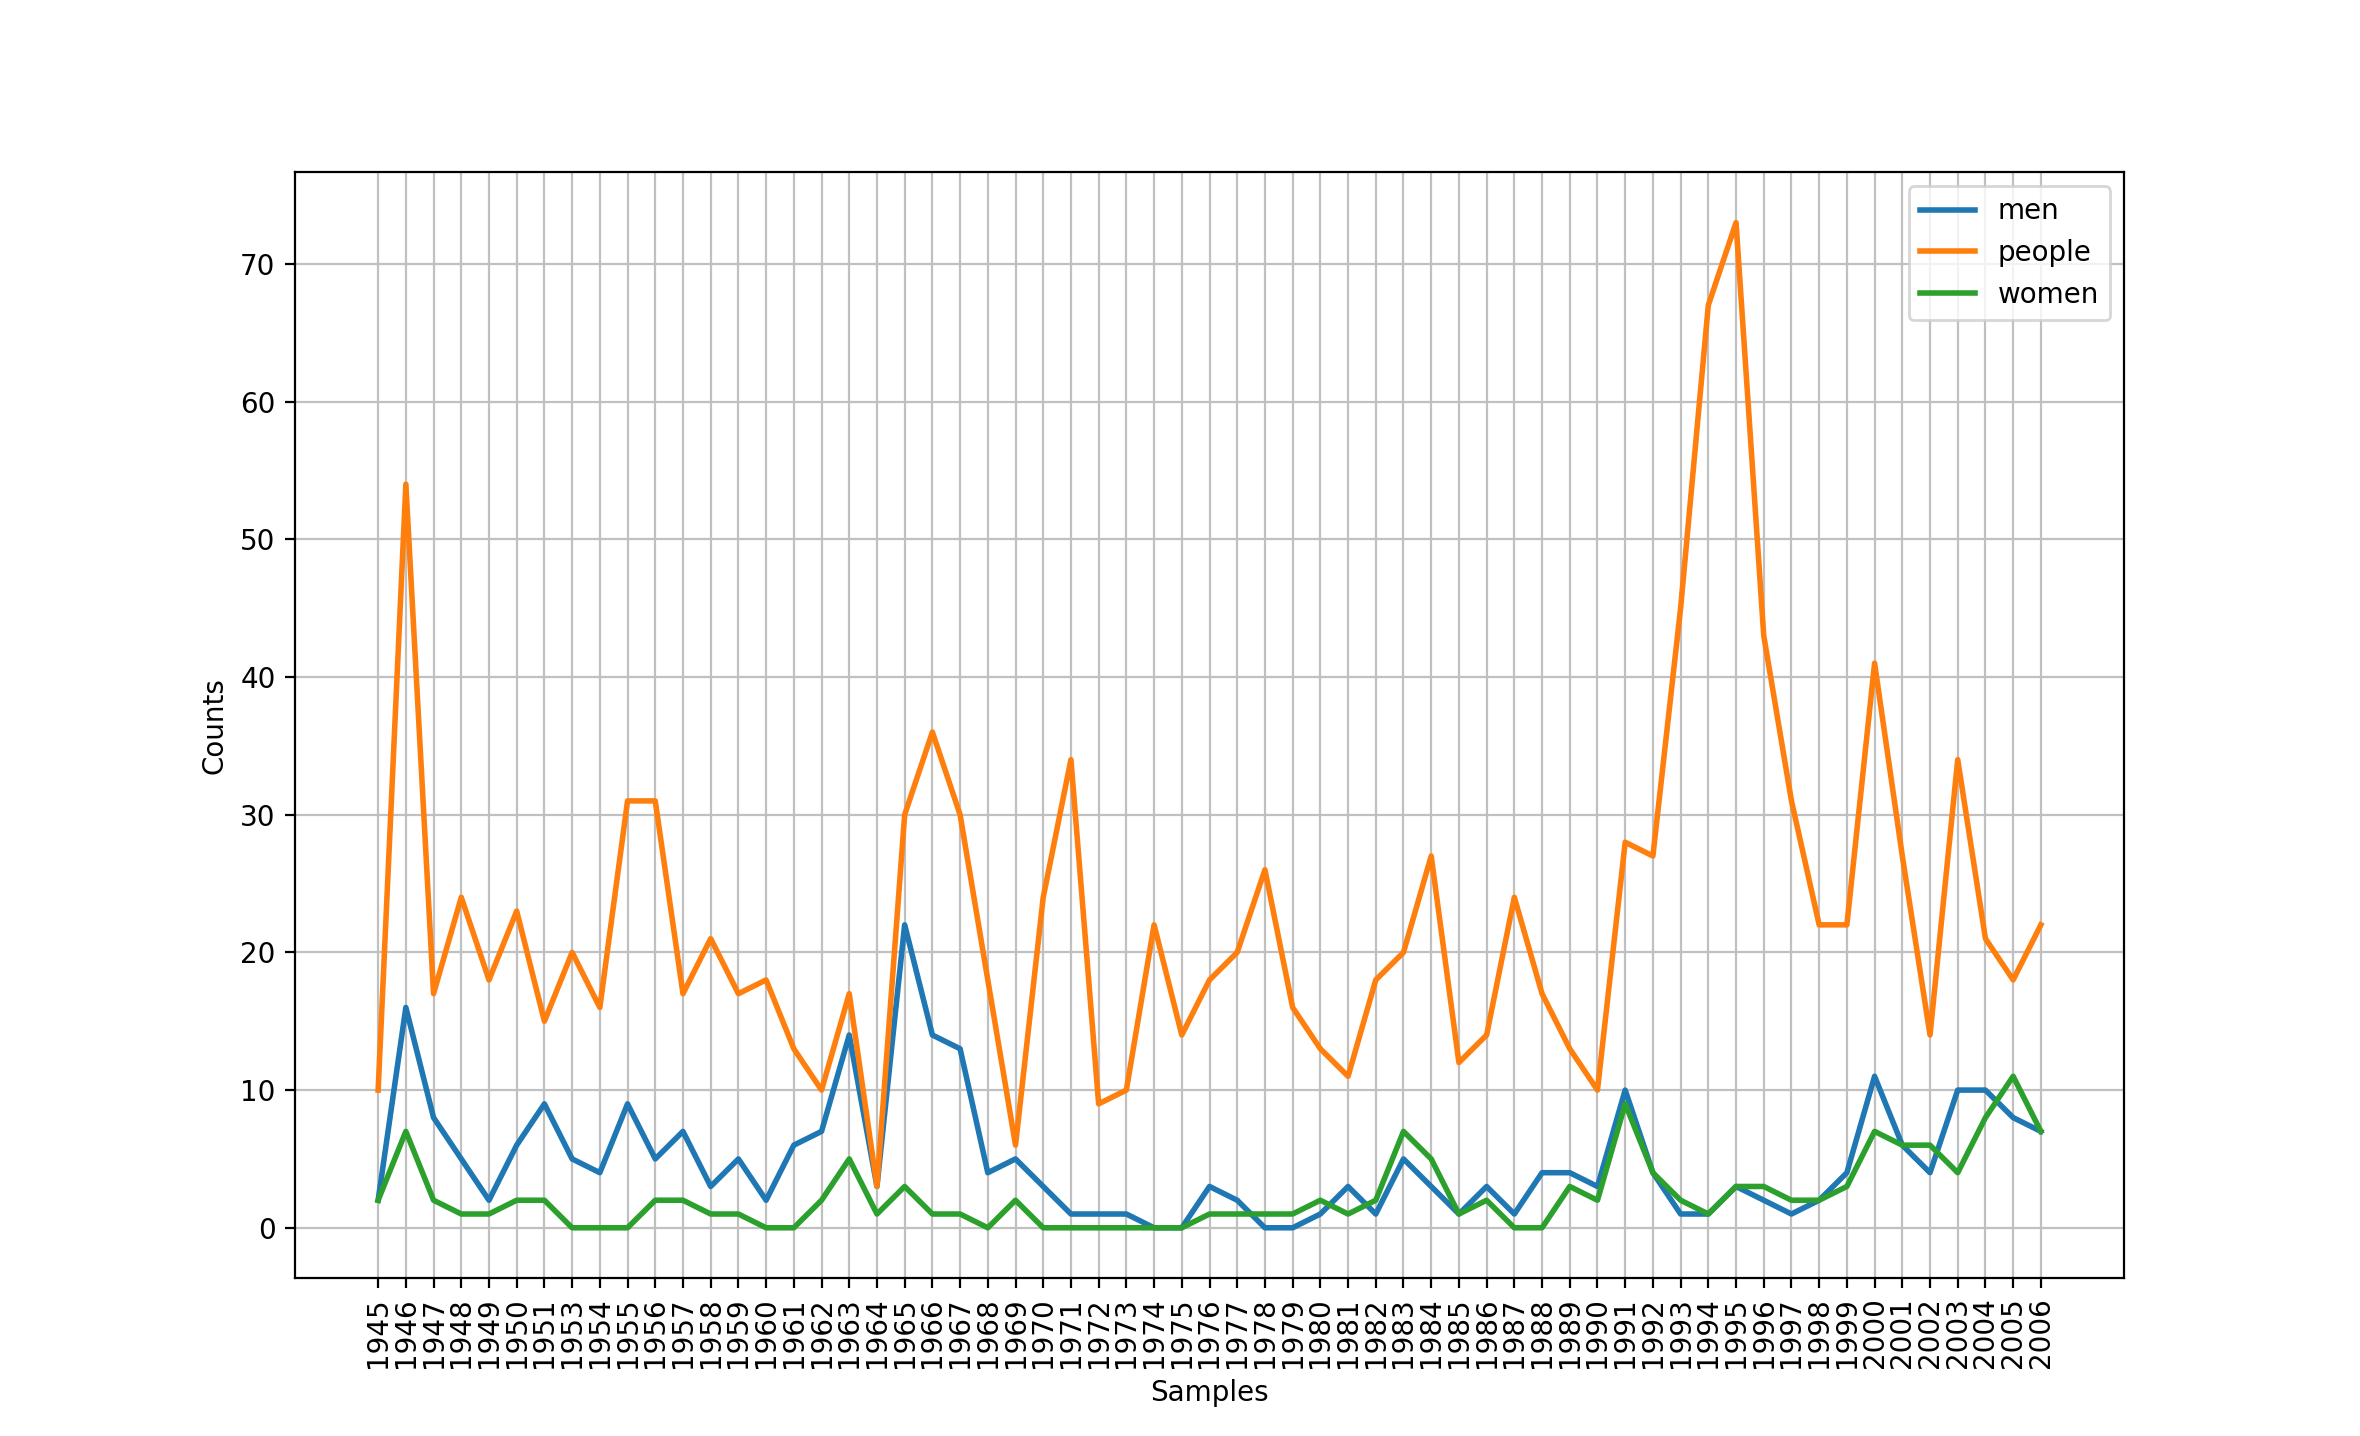
\includegraphics[width=\textwidth]{Figure_1.png}
	
	There appear to be various peaks, but in the most recent two decades, the occurences of "people" appears to decrease, while the occurrences of both "men" and "women" appear to increase.
	
	Code used to generate plot:
	\begin{lstlisting}
	>>> cfd = nltk.ConditionalFreqDist(
	...           (target, fileid[:4])
	...           for fileid in stae_union.fileids()
	...           for w in inaugural.words(fileid)
	...           for target in ['men', 'women', 'people']
	...           if w.lower().startswith(target)) [1]
	>>> cfd.plot()
	\end{lstlisting}
	
\section*{Problem 5} Investigate the \codeword{holonym-meronym} relations for some nouns. Remember that there are three kinds of \codeword{holonym-meronym} relation, so you need to use: \codeword{member_meronyms()}, \codeword{part_meronyms()}, 
	\codeword{substance_meronyms()}, \codeword{member_holonyms()}, \codeword{part_holonyms()}, and \codeword{substance_holonyms()}.
	
	\begin{lstlisting}
	>>> wn.synsets('chair')
	[Synset('chair.n.01'), Synset('professorship.n.01'), Synset('president.n.04'), Synset('electric_chair.n.01'), Synset('chair.n.05'), Synset('chair.v.01'), Synset('moderate.v.01')]
	>>> wn.synset('chair.n.01').substance_holonyms()
	[]
	>>> wn.synset('chair.n.01').part_holonyms()
	[]
	>>> wn.synset('chair.n.01').member_holonyms()
	[]
	>>> wn.synset('chair.n.01').member_meronyms()
	[]
	>>> wn.synset('chair.n.01').substance_meronyms()
	[]
	>>> wn.synset('chair.n.01').part_meronyms()
	[Synset('back.n.08'), Synset('leg.n.03')]
	>>> wn.synsets('leaf')
	[Synset('leaf.n.01'), Synset('leaf.n.02'), Synset('leaf.n.03'), Synset('flick.v.02'), Synset('leaf.v.02'), Synset('leaf.v.03')]
	>>> wn.synset('leaf.n.01').part_meronyms()
	[Synset('leaf_shape.n.01'), Synset('lobe.n.02'), Synset('venation.n.01')]
	>>> wn.synset('chair.n.01').substance_meronyms()
	[]
	>>> wn.synset('chair.n.01').member_meronyms()
	[]
	>>> wn.synset('chair.n.01').member_holonyms()
	[]
	>>> wn.synset('chair.n.01').part_holonyms()
	[]
	>>> wn.synset('chair.n.01').substance_holonyms()
	[]
	\end{lstlisting}
	
\subsection*{Problem 19} Pick a pair of texts and study the differences between them, in terms of vocabulary, vocabulary richness, genre, etc. Can you find pairs of words which have quite different meanings across the two texts, such as monstrous in Moby Dick and in Sense and Sensibility?

\begin{lstlisting}
>>> from nltk.corpus import gutenberg
>>> alice = gutenberg.words('carroll-alice.txt')
>>> paradise = gutenberg.words('milton-paradise.txt')
>>> len(set(alice))
3016
>>> len(set(paradise))
10751
>>> len(set(alice)) / len(alice)
0.08841981823512167
>>> len(set(paradise)) / len(paradise)
0.11103537309579138

>>> alice.concordance("heavy")
Displaying 2 of 2 matches:
from the Gryphon , and the constant heavy sobbing of the Mock Turtle . Alice w
ake the place of the Mock Turtle s heavy sobs . Lastly , she pictured to hers
>>> paradise.concordance("heavy")
Displaying 5 of 5 matches:
eir several clans , Light - armed or heavy , sharp , smooth , swift , or slow ,
: When behold ! Not distant far with heavy pace the foe Approaching gross and h
, as on their natural center , light Heavy , though in their place . O fleeting
hame Done to his father , heard this heavy curse , Servant of servants , on his
ble ? yet many will presume : Whence heavy persecution shall arise On all , who
\end{lstlisting}

In Alice in Wonderland, the word "heavy" describes powerful sobs both times it is used. However, in Paradise Lost, heavy descripts the pace of a character's gait, or the weight of a curse or persecution. Both describe the power behind an object, but in different contexts.

\begin{lstlisting}
>>> alice.concordance("dream")
Displaying 7 of 7 matches:
s dozing off , and had just begun to dream that she was walking hand in hand wi
!' ' Oh , I ' ve had such a curious dream !' said Alice , and she told her sis
her , and said , ' It WAS a curious dream , dear , certainly : but now run in
as well she might , what a wonderful dream it had been . But her sister sat sti
g after a fashion , and this was her dream :-- First , she dreamed of little Al
e creatures of her little sister ' s dream . The long grass rustled at her feet
strange tale , perhaps even with the dream of Wonderland of long ago : and how
>>> paradise.concordance("dream")
Displaying 12 of 12 matches:
rowing empire ; doubtless ! while we dream , And know not that the King of Heav
how glad I waked To find this but a dream ! Thus Eve her night Related , and t
qually ; nor can I like This uncouth dream , of evil sprung , I fear ; Yet evil
last evening s talk , in this thy dream , But with addition strange ; yet be
at what in sleep thou didst abhor to dream , Waking thou never will consent to
For thou art heavenly , she an empty dream . Say , Goddess , what ensued when R
what concerns thee , and thy being ; Dream not of other worlds , what creatures
e : When suddenly stood at my head a dream , Whose inward apparition gently mov
d Before mine eyes all real , as the dream Had lively shadowed : Here had new b
ot far off , Such as I saw her in my dream , adorned With what all Earth or Hea
life , and eat , And live for ever , dream at least to live For ever , to remov
or s heel . To whom thus Michael . Dream not of their fight , As of a duel ,
\end{lstlisting}
	Similarly, both texts reference the 'dream' but in very different contexts. In Alice in Wonderland, Alice talks of 'curious' and 'wonderful' dreams, describing the fantastic nature of her adventure. In Paradise Lost, 'dream'  references either hope ('dream not of their fight', 'dream not of other worlds') or the nightmare quality of the situation ('empty dream' , 'uncouth dream')
	
	
\subsection*{Problem 23} Zipf's Law: Let f(w) be the frequency of a word w in free text. Suppose that all the words of a text are ranked according to their frequency, with the most frequent word first. Zipf's law states that the frequency of a word type is inversely proportional to its rank (i.e. f × r = k, for some constant k). For example, the 50th most common word type should occur three times as frequently as the 150th most common word type.

\begin{enumerate}
	\item Write a function to process a large text and plot word frequency against word rank using pylab.plot. Do you confirm Zipf's law? (Hint: it helps to use a logarithmic scale). What is going on at the extreme ends of the plotted line?
	
	\item Generate random text, e.g., using random.choice("abcdefg "), taking care to include the space character. You will need to import random first. Use the string concatenation operator to accumulate characters into a (very) long string. Then tokenize this string, and generate the Zipf plot as before, and compare the two plots. What do you make of Zipf's Law in the light of this?
\end{enumerate}

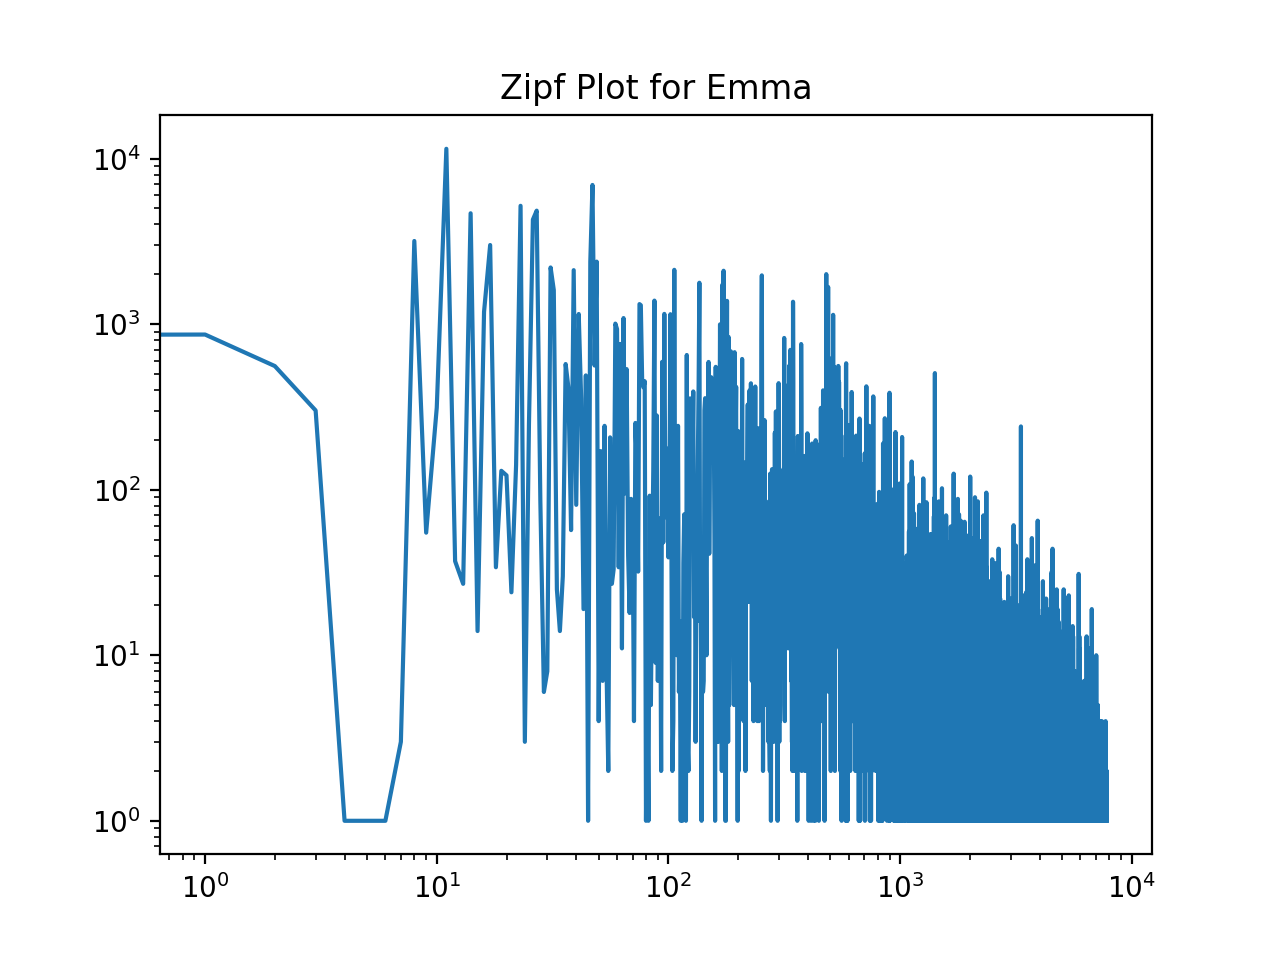
\includegraphics[scale=0.7]{ZipfEmma.png}\\

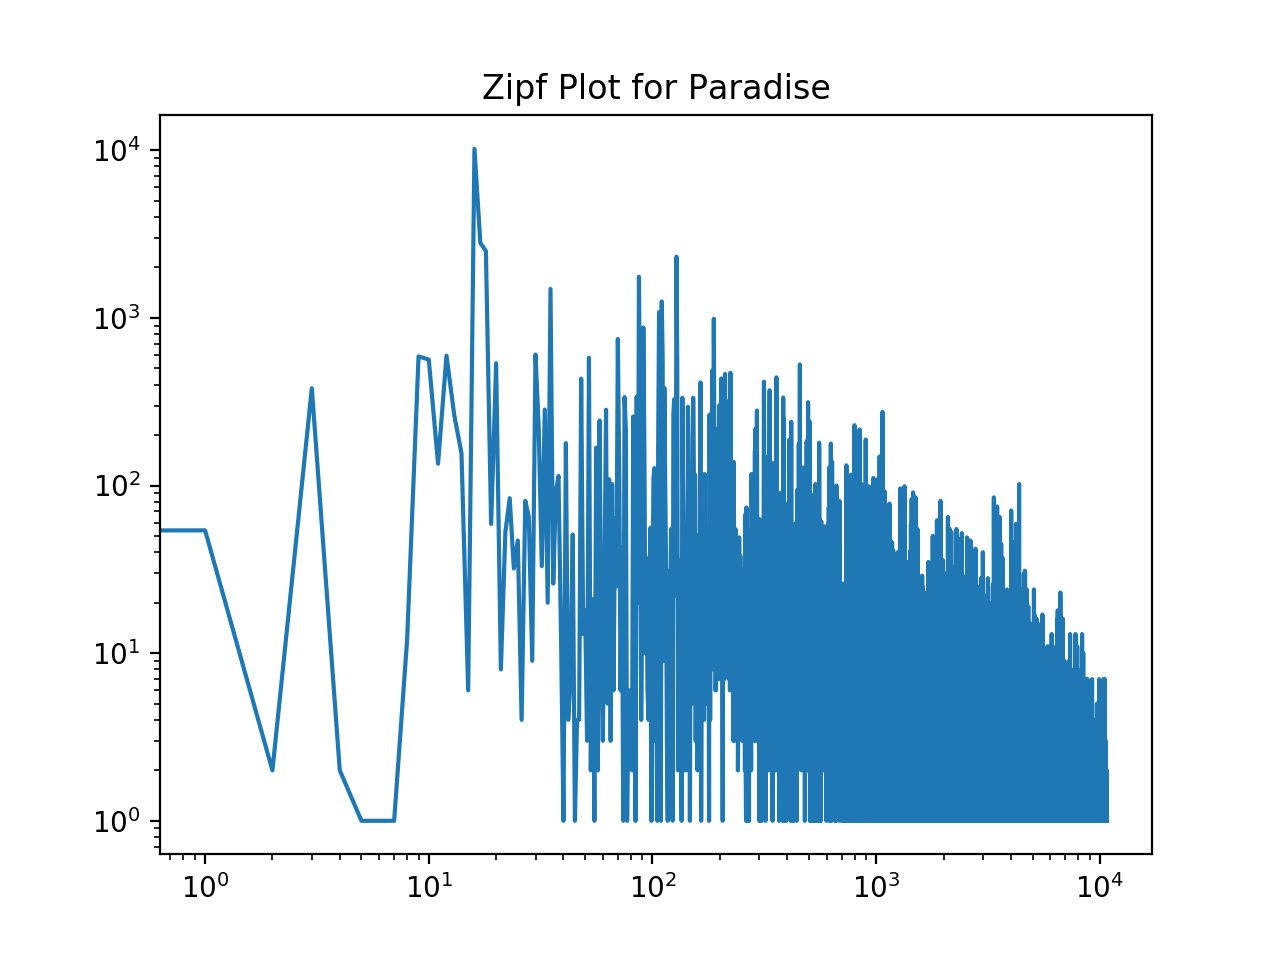
\includegraphics[scale=0.7]{ZipfParadise.png}\\
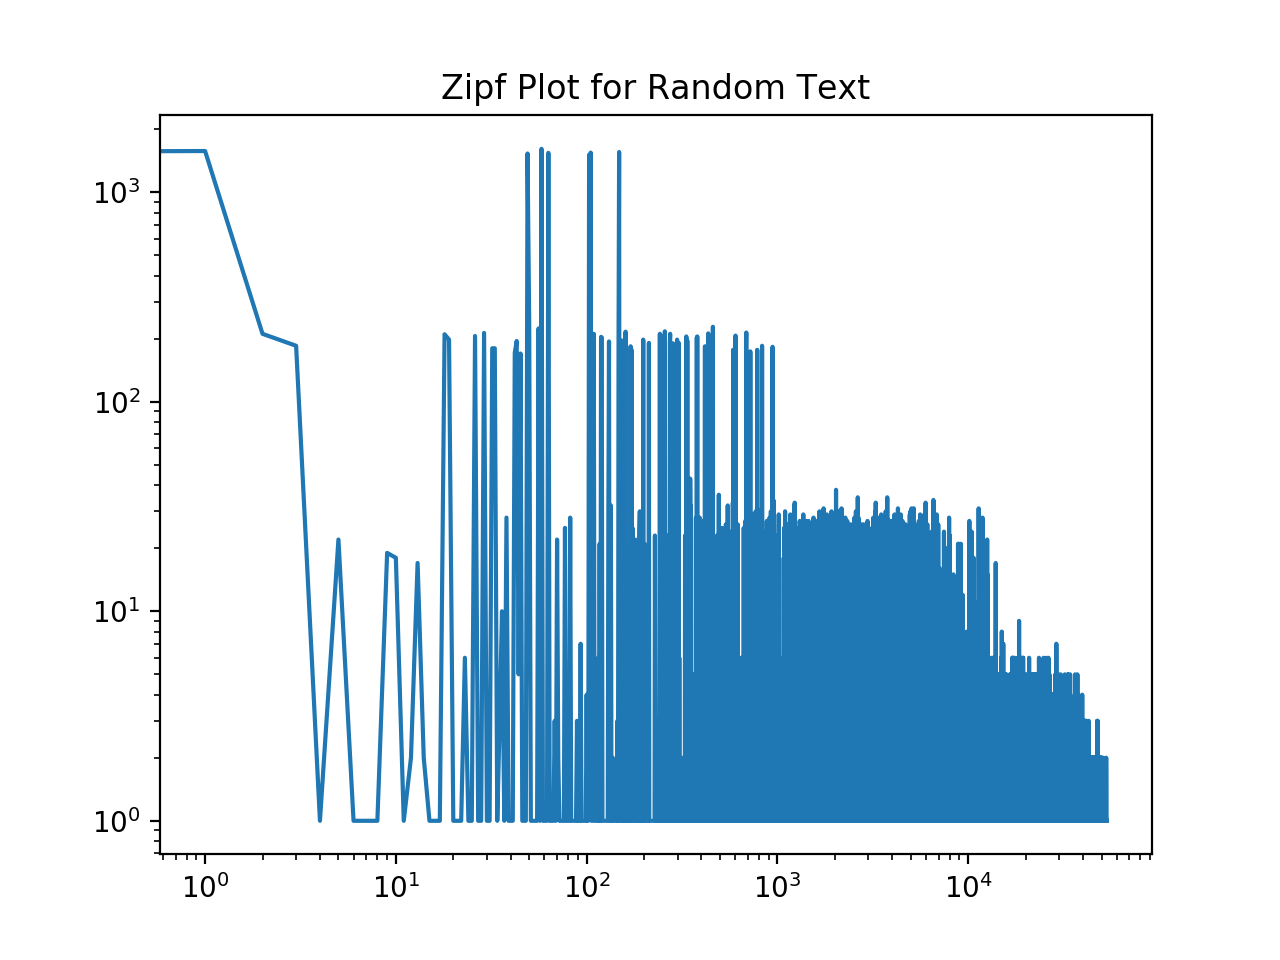
\includegraphics[scale=0.7]{ZipfRandom.png}\\

All the Zipf plots I generated (for both input texts from the gutenberg corpus and the random text) all appear to have a similar shape, and look approximately linear in the middle. My observations and the above plots corroborate Zipf's law. The full module I wrote to generate the plots is attached in a pdf.

\section*{Part II}
Identify a recent research publication that interests you. Write a very short summary and explain why you found it interesting. Be prepared to discuss this in class next week. 

A research publication in which I am especially intersted is The Stanford Natural Language Processing Group (https://nlp.stanford.edu/pubs/). Standford is the preiminent machine learning research university, and the are often the paragon of innovative techniques. 
	

\end{document}